\documentclass{article}
\usepackage{tikz}
\usetikzlibrary{arrows.meta, positioning}

\begin{document}

\begin{figure}[h]
    \centering
    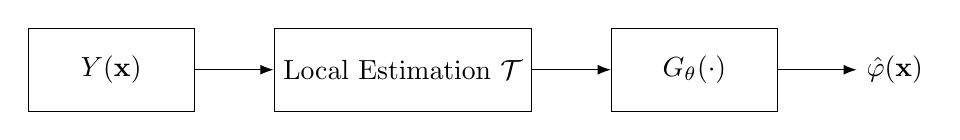
\begin{tikzpicture}[node distance=1cm, auto,
        block/.style={draw, rectangle, minimum height=3em, minimum width=6em},
        line/.style={draw, -Latex}]
        
        % Nodes
        \node [block] (input) {$Y(\mathbf{x})$};
        \node [block, right=of input] (estimation) {Local Estimation $\mathcal{T}$};
        \node [block, right=of estimation] (neural_network) {$G_\theta(\cdot)$};
        \node [right=of neural_network] (output) {$\hat{\varphi}(\mathbf{x})$};
        
        % Arrows
        \path [line] (input) -- (estimation);
        \path [line] (estimation) -- (neural_network);
        \path [line] (neural_network) -- (output);
        
    \end{tikzpicture}
    
    \caption{Data processing pipeline: we first perform an initial and simple estimation on $Y(\mathbf{x})$, generating the initial estimate $\tilde{\varphi}(\mathbf{x})$; then, we use a neural network to refine it, producing the final estimate $\hat{\varphi}(\mathbf{x})$.}
    \label{fig:data_pipeline}
\end{figure}

\end{document}